% Options for packages loaded elsewhere
\PassOptionsToPackage{unicode}{hyperref}
\PassOptionsToPackage{hyphens}{url}
%
\documentclass[
]{article}
\usepackage{amsmath,amssymb}
\usepackage{lmodern}
\usepackage{ifxetex,ifluatex}
\ifnum 0\ifxetex 1\fi\ifluatex 1\fi=0 % if pdftex
  \usepackage[T1]{fontenc}
  \usepackage[utf8]{inputenc}
  \usepackage{textcomp} % provide euro and other symbols
\else % if luatex or xetex
  \usepackage{unicode-math}
  \defaultfontfeatures{Scale=MatchLowercase}
  \defaultfontfeatures[\rmfamily]{Ligatures=TeX,Scale=1}
\fi
% Use upquote if available, for straight quotes in verbatim environments
\IfFileExists{upquote.sty}{\usepackage{upquote}}{}
\IfFileExists{microtype.sty}{% use microtype if available
  \usepackage[]{microtype}
  \UseMicrotypeSet[protrusion]{basicmath} % disable protrusion for tt fonts
}{}
\makeatletter
\@ifundefined{KOMAClassName}{% if non-KOMA class
  \IfFileExists{parskip.sty}{%
    \usepackage{parskip}
  }{% else
    \setlength{\parindent}{0pt}
    \setlength{\parskip}{6pt plus 2pt minus 1pt}}
}{% if KOMA class
  \KOMAoptions{parskip=half}}
\makeatother
\usepackage{xcolor}
\IfFileExists{xurl.sty}{\usepackage{xurl}}{} % add URL line breaks if available
\IfFileExists{bookmark.sty}{\usepackage{bookmark}}{\usepackage{hyperref}}
\hypersetup{
  pdftitle={Harrison Montoya Assignments},
  hidelinks,
  pdfcreator={LaTeX via pandoc}}
\urlstyle{same} % disable monospaced font for URLs
\usepackage[margin=1in]{geometry}
\usepackage{color}
\usepackage{fancyvrb}
\newcommand{\VerbBar}{|}
\newcommand{\VERB}{\Verb[commandchars=\\\{\}]}
\DefineVerbatimEnvironment{Highlighting}{Verbatim}{commandchars=\\\{\}}
% Add ',fontsize=\small' for more characters per line
\usepackage{framed}
\definecolor{shadecolor}{RGB}{248,248,248}
\newenvironment{Shaded}{\begin{snugshade}}{\end{snugshade}}
\newcommand{\AlertTok}[1]{\textcolor[rgb]{0.94,0.16,0.16}{#1}}
\newcommand{\AnnotationTok}[1]{\textcolor[rgb]{0.56,0.35,0.01}{\textbf{\textit{#1}}}}
\newcommand{\AttributeTok}[1]{\textcolor[rgb]{0.77,0.63,0.00}{#1}}
\newcommand{\BaseNTok}[1]{\textcolor[rgb]{0.00,0.00,0.81}{#1}}
\newcommand{\BuiltInTok}[1]{#1}
\newcommand{\CharTok}[1]{\textcolor[rgb]{0.31,0.60,0.02}{#1}}
\newcommand{\CommentTok}[1]{\textcolor[rgb]{0.56,0.35,0.01}{\textit{#1}}}
\newcommand{\CommentVarTok}[1]{\textcolor[rgb]{0.56,0.35,0.01}{\textbf{\textit{#1}}}}
\newcommand{\ConstantTok}[1]{\textcolor[rgb]{0.00,0.00,0.00}{#1}}
\newcommand{\ControlFlowTok}[1]{\textcolor[rgb]{0.13,0.29,0.53}{\textbf{#1}}}
\newcommand{\DataTypeTok}[1]{\textcolor[rgb]{0.13,0.29,0.53}{#1}}
\newcommand{\DecValTok}[1]{\textcolor[rgb]{0.00,0.00,0.81}{#1}}
\newcommand{\DocumentationTok}[1]{\textcolor[rgb]{0.56,0.35,0.01}{\textbf{\textit{#1}}}}
\newcommand{\ErrorTok}[1]{\textcolor[rgb]{0.64,0.00,0.00}{\textbf{#1}}}
\newcommand{\ExtensionTok}[1]{#1}
\newcommand{\FloatTok}[1]{\textcolor[rgb]{0.00,0.00,0.81}{#1}}
\newcommand{\FunctionTok}[1]{\textcolor[rgb]{0.00,0.00,0.00}{#1}}
\newcommand{\ImportTok}[1]{#1}
\newcommand{\InformationTok}[1]{\textcolor[rgb]{0.56,0.35,0.01}{\textbf{\textit{#1}}}}
\newcommand{\KeywordTok}[1]{\textcolor[rgb]{0.13,0.29,0.53}{\textbf{#1}}}
\newcommand{\NormalTok}[1]{#1}
\newcommand{\OperatorTok}[1]{\textcolor[rgb]{0.81,0.36,0.00}{\textbf{#1}}}
\newcommand{\OtherTok}[1]{\textcolor[rgb]{0.56,0.35,0.01}{#1}}
\newcommand{\PreprocessorTok}[1]{\textcolor[rgb]{0.56,0.35,0.01}{\textit{#1}}}
\newcommand{\RegionMarkerTok}[1]{#1}
\newcommand{\SpecialCharTok}[1]{\textcolor[rgb]{0.00,0.00,0.00}{#1}}
\newcommand{\SpecialStringTok}[1]{\textcolor[rgb]{0.31,0.60,0.02}{#1}}
\newcommand{\StringTok}[1]{\textcolor[rgb]{0.31,0.60,0.02}{#1}}
\newcommand{\VariableTok}[1]{\textcolor[rgb]{0.00,0.00,0.00}{#1}}
\newcommand{\VerbatimStringTok}[1]{\textcolor[rgb]{0.31,0.60,0.02}{#1}}
\newcommand{\WarningTok}[1]{\textcolor[rgb]{0.56,0.35,0.01}{\textbf{\textit{#1}}}}
\usepackage{graphicx}
\makeatletter
\def\maxwidth{\ifdim\Gin@nat@width>\linewidth\linewidth\else\Gin@nat@width\fi}
\def\maxheight{\ifdim\Gin@nat@height>\textheight\textheight\else\Gin@nat@height\fi}
\makeatother
% Scale images if necessary, so that they will not overflow the page
% margins by default, and it is still possible to overwrite the defaults
% using explicit options in \includegraphics[width, height, ...]{}
\setkeys{Gin}{width=\maxwidth,height=\maxheight,keepaspectratio}
% Set default figure placement to htbp
\makeatletter
\def\fps@figure{htbp}
\makeatother
\setlength{\emergencystretch}{3em} % prevent overfull lines
\providecommand{\tightlist}{%
  \setlength{\itemsep}{0pt}\setlength{\parskip}{0pt}}
\setcounter{secnumdepth}{-\maxdimen} % remove section numbering
\ifluatex
  \usepackage{selnolig}  % disable illegal ligatures
\fi

\title{Harrison Montoya Assignments}
\author{}
\date{\vspace{-2.5em}}

\begin{document}
\maketitle

\hypertarget{assignment-1}{%
\section{Assignment 1}\label{assignment-1}}

Due on Canvas on Monday 9/20 before class, at 10:15 am.

\hypertarget{problem-1}{%
\subsubsection{Problem 1}\label{problem-1}}

Install the datasets package on the console below using
\texttt{install.packages("datasets")}. Now load the library.

\begin{Shaded}
\begin{Highlighting}[]
\NormalTok{USArrests}
\end{Highlighting}
\end{Shaded}

\begin{verbatim}
##                Murder Assault UrbanPop Rape
## Alabama          13.2     236       58 21.2
## Alaska           10.0     263       48 44.5
## Arizona           8.1     294       80 31.0
## Arkansas          8.8     190       50 19.5
## California        9.0     276       91 40.6
## Colorado          7.9     204       78 38.7
## Connecticut       3.3     110       77 11.1
## Delaware          5.9     238       72 15.8
## Florida          15.4     335       80 31.9
## Georgia          17.4     211       60 25.8
## Hawaii            5.3      46       83 20.2
## Idaho             2.6     120       54 14.2
## Illinois         10.4     249       83 24.0
## Indiana           7.2     113       65 21.0
## Iowa              2.2      56       57 11.3
## Kansas            6.0     115       66 18.0
## Kentucky          9.7     109       52 16.3
## Louisiana        15.4     249       66 22.2
## Maine             2.1      83       51  7.8
## Maryland         11.3     300       67 27.8
## Massachusetts     4.4     149       85 16.3
## Michigan         12.1     255       74 35.1
## Minnesota         2.7      72       66 14.9
## Mississippi      16.1     259       44 17.1
## Missouri          9.0     178       70 28.2
## Montana           6.0     109       53 16.4
## Nebraska          4.3     102       62 16.5
## Nevada           12.2     252       81 46.0
## New Hampshire     2.1      57       56  9.5
## New Jersey        7.4     159       89 18.8
## New Mexico       11.4     285       70 32.1
## New York         11.1     254       86 26.1
## North Carolina   13.0     337       45 16.1
## North Dakota      0.8      45       44  7.3
## Ohio              7.3     120       75 21.4
## Oklahoma          6.6     151       68 20.0
## Oregon            4.9     159       67 29.3
## Pennsylvania      6.3     106       72 14.9
## Rhode Island      3.4     174       87  8.3
## South Carolina   14.4     279       48 22.5
## South Dakota      3.8      86       45 12.8
## Tennessee        13.2     188       59 26.9
## Texas            12.7     201       80 25.5
## Utah              3.2     120       80 22.9
## Vermont           2.2      48       32 11.2
## Virginia          8.5     156       63 20.7
## Washington        4.0     145       73 26.2
## West Virginia     5.7      81       39  9.3
## Wisconsin         2.6      53       66 10.8
## Wyoming           6.8     161       60 15.6
\end{verbatim}

Load the USArrests dataset and rename it \texttt{dat}. Note that this
dataset comes with R, in the package datasets, so there's no need to
load data from your computer. Why is it useful to rename the dataset?

\begin{Shaded}
\begin{Highlighting}[]
\NormalTok{dat}\OtherTok{\textless{}{-}}\NormalTok{USArrests}
\NormalTok{dat.USArrests }\OtherTok{\textless{}{-}}\NormalTok{ dat}
\end{Highlighting}
\end{Shaded}

\emph{Answer:} It is useful to rename the dataset for two reasons.
First, it will help you keep track of your work and not confuse it with
other generic-looking names of other datasets. Second, it will allow you
to keep an original copy of the file while creating a new file with all
of the changes you are currently making on it.

\hypertarget{problem-2}{%
\subsubsection{Problem 2}\label{problem-2}}

Use this command to make the state names into a new variable called
State.

\begin{Shaded}
\begin{Highlighting}[]
\NormalTok{dat.USArrests}\SpecialCharTok{$}\NormalTok{state }\OtherTok{\textless{}{-}} \FunctionTok{tolower}\NormalTok{(}\FunctionTok{rownames}\NormalTok{(USArrests))}
\NormalTok{dat.USArrests}
\end{Highlighting}
\end{Shaded}

\begin{verbatim}
##                Murder Assault UrbanPop Rape          state
## Alabama          13.2     236       58 21.2        alabama
## Alaska           10.0     263       48 44.5         alaska
## Arizona           8.1     294       80 31.0        arizona
## Arkansas          8.8     190       50 19.5       arkansas
## California        9.0     276       91 40.6     california
## Colorado          7.9     204       78 38.7       colorado
## Connecticut       3.3     110       77 11.1    connecticut
## Delaware          5.9     238       72 15.8       delaware
## Florida          15.4     335       80 31.9        florida
## Georgia          17.4     211       60 25.8        georgia
## Hawaii            5.3      46       83 20.2         hawaii
## Idaho             2.6     120       54 14.2          idaho
## Illinois         10.4     249       83 24.0       illinois
## Indiana           7.2     113       65 21.0        indiana
## Iowa              2.2      56       57 11.3           iowa
## Kansas            6.0     115       66 18.0         kansas
## Kentucky          9.7     109       52 16.3       kentucky
## Louisiana        15.4     249       66 22.2      louisiana
## Maine             2.1      83       51  7.8          maine
## Maryland         11.3     300       67 27.8       maryland
## Massachusetts     4.4     149       85 16.3  massachusetts
## Michigan         12.1     255       74 35.1       michigan
## Minnesota         2.7      72       66 14.9      minnesota
## Mississippi      16.1     259       44 17.1    mississippi
## Missouri          9.0     178       70 28.2       missouri
## Montana           6.0     109       53 16.4        montana
## Nebraska          4.3     102       62 16.5       nebraska
## Nevada           12.2     252       81 46.0         nevada
## New Hampshire     2.1      57       56  9.5  new hampshire
## New Jersey        7.4     159       89 18.8     new jersey
## New Mexico       11.4     285       70 32.1     new mexico
## New York         11.1     254       86 26.1       new york
## North Carolina   13.0     337       45 16.1 north carolina
## North Dakota      0.8      45       44  7.3   north dakota
## Ohio              7.3     120       75 21.4           ohio
## Oklahoma          6.6     151       68 20.0       oklahoma
## Oregon            4.9     159       67 29.3         oregon
## Pennsylvania      6.3     106       72 14.9   pennsylvania
## Rhode Island      3.4     174       87  8.3   rhode island
## South Carolina   14.4     279       48 22.5 south carolina
## South Dakota      3.8      86       45 12.8   south dakota
## Tennessee        13.2     188       59 26.9      tennessee
## Texas            12.7     201       80 25.5          texas
## Utah              3.2     120       80 22.9           utah
## Vermont           2.2      48       32 11.2        vermont
## Virginia          8.5     156       63 20.7       virginia
## Washington        4.0     145       73 26.2     washington
## West Virginia     5.7      81       39  9.3  west virginia
## Wisconsin         2.6      53       66 10.8      wisconsin
## Wyoming           6.8     161       60 15.6        wyoming
\end{verbatim}

This dataset has the state names as row names, so we just want to make
them into a new variable. We also make them all lower case, because that
will help us draw a map later - the map function requires the states to
be lower case.

List the variables contained in the dataset \texttt{USArrests}.

\begin{Shaded}
\begin{Highlighting}[]
\FunctionTok{names}\NormalTok{(dat.USArrests)}
\end{Highlighting}
\end{Shaded}

\begin{verbatim}
## [1] "Murder"   "Assault"  "UrbanPop" "Rape"     "state"
\end{verbatim}

\emph{Answer:} The variables include Murder, Assault, Rape, Urban
Population, and State.

\hypertarget{problem-3}{%
\subsubsection{Problem 3}\label{problem-3}}

What type of variable (from the DVB chapter) is \texttt{Murder}?

\emph{Answer:} In the DVB chapter, ``Murder'' would be considered a
qualitative, or categorical, variable.

What R Type of variable is it?

\emph{Answer:} ``Murder'' is considered a character in R.

\hypertarget{problem-4}{%
\subsubsection{Problem 4}\label{problem-4}}

What information is contained in this dataset, in general? What do the
numbers mean?

\emph{Answer:} The dataset includes the arrest rates for murder,
assault, and rape per 100,000 residents in each of the US's 50 states.
Additionally, the percent of the population living in urban areas is
given. Here, then, the numbers mean either the arrest rates for a crime
per 100k residents in a state or the percent of residents living in
urban spaces in a state.

\hypertarget{problem-5}{%
\subsubsection{Problem 5}\label{problem-5}}

Draw a histogram of \texttt{Murder} with proper labels and title.

\begin{Shaded}
\begin{Highlighting}[]
\FunctionTok{hist}\NormalTok{(dat.USArrests}\SpecialCharTok{$}\NormalTok{Murder, }\AttributeTok{main=}\StringTok{"Histogram of Murder Rates"}\NormalTok{, }\AttributeTok{xlab=}\StringTok{"Murder Rates per State"}\NormalTok{, }\AttributeTok{ylab=}\StringTok{"Frequency"}\NormalTok{)}
\end{Highlighting}
\end{Shaded}

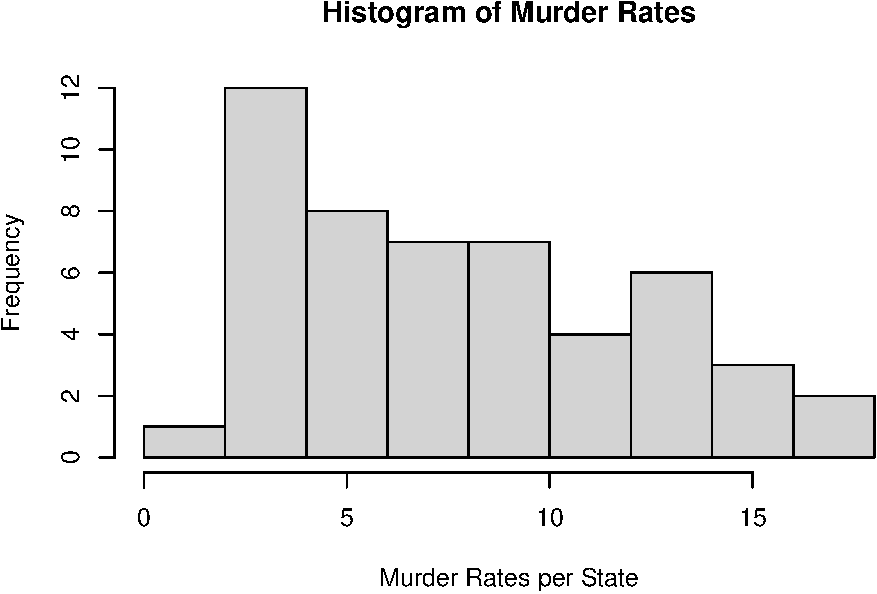
\includegraphics{Assignment-1-HarrisonMontoya_files/figure-latex/unnamed-chunk-5-1.pdf}

\hypertarget{problem-6}{%
\subsubsection{Problem 6}\label{problem-6}}

Please summarize \texttt{Murder} quantitatively. What are its mean and
median? What is the difference between mean and median? What is a
quartile, and why do you think R gives you the 1st Qu. and 3rd Qu.?

\begin{Shaded}
\begin{Highlighting}[]
\FunctionTok{summary}\NormalTok{(dat.USArrests}\SpecialCharTok{$}\NormalTok{Murder)}
\end{Highlighting}
\end{Shaded}

\begin{verbatim}
##    Min. 1st Qu.  Median    Mean 3rd Qu.    Max. 
##   0.800   4.075   7.250   7.788  11.250  17.400
\end{verbatim}

\emph{Answer:} The mean of ``Murder'' is 7.788, while its median is
7.250. Generally, mean signifies the solution of all of the values added
together and then divided by the number of values, while median
signifies the middle value when all values are lined up in ascending
order. A quartile constitutes one of three values that divides a data
distribution into fourths. Lastly, R would provide the first and third
quartile in order to help the statistician understand where the majority
of values lie (in between the first and third quartile) or what values
might be considered outliers (before the first and after the third).

\hypertarget{problem-7}{%
\subsubsection{Problem 7}\label{problem-7}}

Repeat the same steps you followed for \texttt{Murder}, for the
variables \texttt{Assault} and \texttt{Rape}. Now plot all three
histograms together. You can do this by using the command
\texttt{par(mfrow=c(3,1))} and then plotting each of the three.

\begin{Shaded}
\begin{Highlighting}[]
\FunctionTok{hist}\NormalTok{(dat.USArrests}\SpecialCharTok{$}\NormalTok{Assault, }\AttributeTok{main=}\StringTok{"Histogram of Assault Rates"}\NormalTok{, }\AttributeTok{xlab=}\StringTok{"Assault Rates per State"}\NormalTok{, }\AttributeTok{ylab=}\StringTok{"Frequency"}\NormalTok{)}
\end{Highlighting}
\end{Shaded}

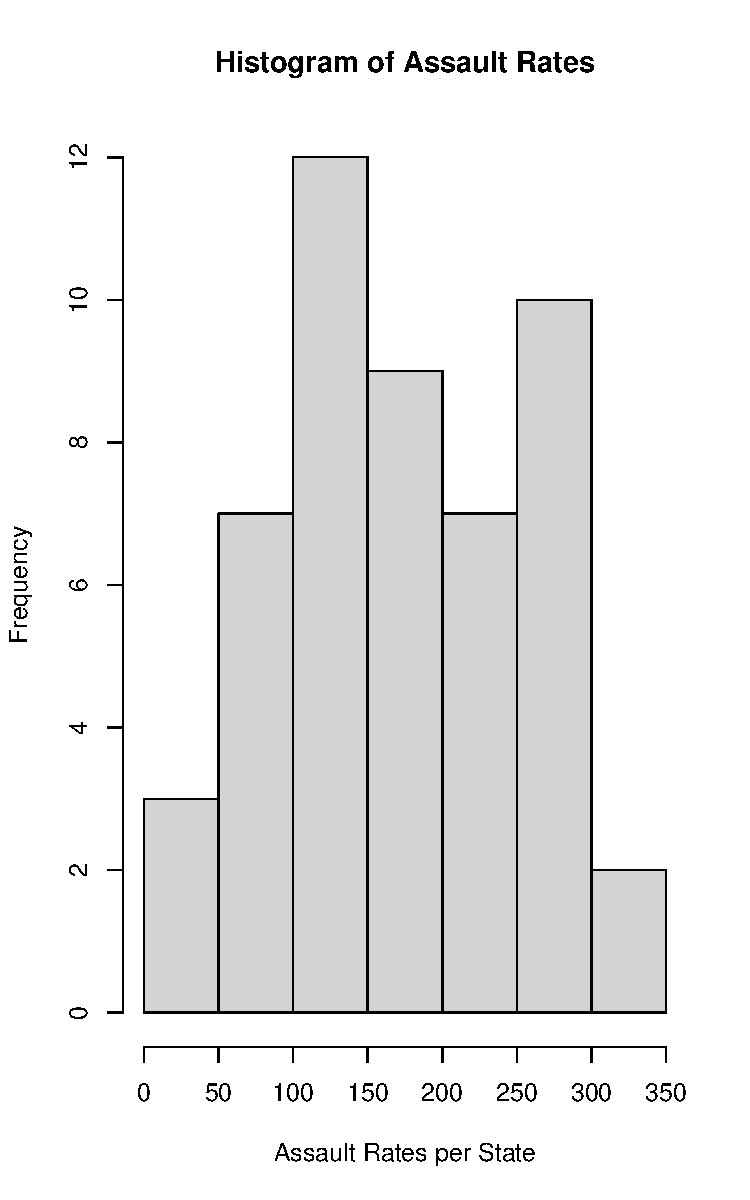
\includegraphics{Assignment-1-HarrisonMontoya_files/figure-latex/unnamed-chunk-7-1.pdf}

\begin{Shaded}
\begin{Highlighting}[]
\FunctionTok{hist}\NormalTok{(dat.USArrests}\SpecialCharTok{$}\NormalTok{Rape, }\AttributeTok{main=}\StringTok{"Histogram of Rape Rates"}\NormalTok{, }\AttributeTok{xlab=}\StringTok{"Rape Rates per State"}\NormalTok{, }\AttributeTok{ylab=}\StringTok{"Frequency"}\NormalTok{)}
\end{Highlighting}
\end{Shaded}

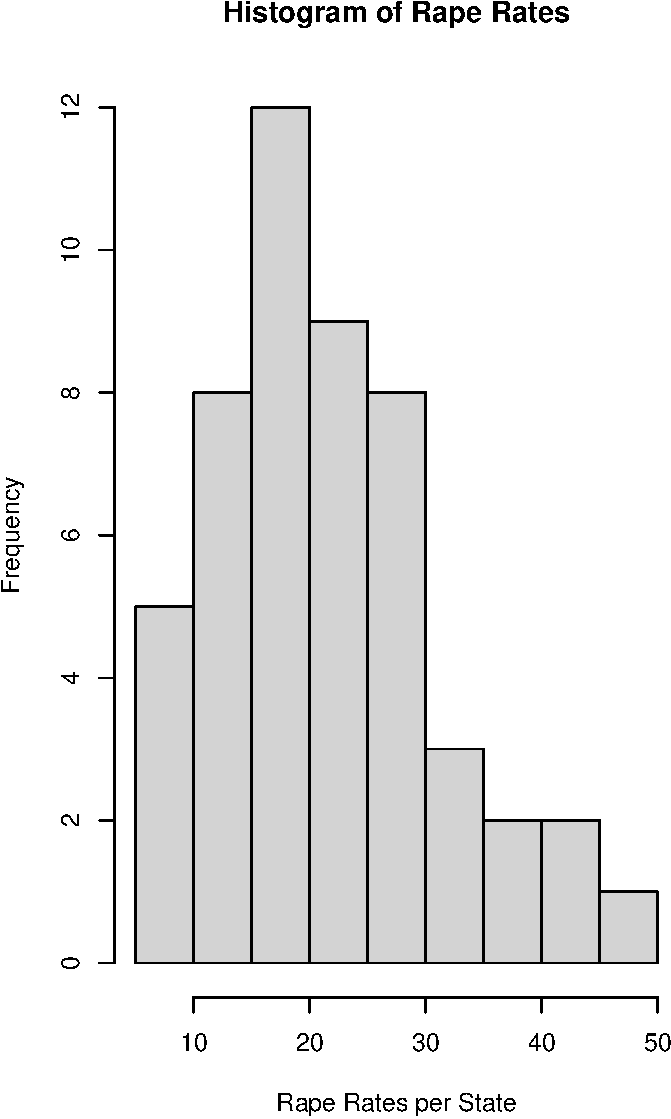
\includegraphics{Assignment-1-HarrisonMontoya_files/figure-latex/unnamed-chunk-7-2.pdf}

\begin{Shaded}
\begin{Highlighting}[]
\FunctionTok{par}\NormalTok{(}\AttributeTok{mfrow=}\FunctionTok{c}\NormalTok{(}\DecValTok{3}\NormalTok{,}\DecValTok{1}\NormalTok{))}
\FunctionTok{hist}\NormalTok{(dat.USArrests}\SpecialCharTok{$}\NormalTok{Murder, }\AttributeTok{main=}\StringTok{"Histogram of Murder Rates"}\NormalTok{, }\AttributeTok{xlab=}\StringTok{"Murder Rates per State"}\NormalTok{, }\AttributeTok{ylab=}\StringTok{"Frequency"}\NormalTok{)}
\FunctionTok{hist}\NormalTok{(dat.USArrests}\SpecialCharTok{$}\NormalTok{Assault, }\AttributeTok{main=}\StringTok{"Histogram of Assault Rates"}\NormalTok{, }\AttributeTok{xlab=}\StringTok{"Assault Rates per State"}\NormalTok{, }\AttributeTok{ylab=}\StringTok{"Frequency"}\NormalTok{)}
\FunctionTok{hist}\NormalTok{(dat.USArrests}\SpecialCharTok{$}\NormalTok{Rape, }\AttributeTok{main=}\StringTok{"Histogram of Rape Rates"}\NormalTok{, }\AttributeTok{xlab=}\StringTok{"Rape Rates per State"}\NormalTok{, }\AttributeTok{ylab=}\StringTok{"Frequency"}\NormalTok{)}
\end{Highlighting}
\end{Shaded}

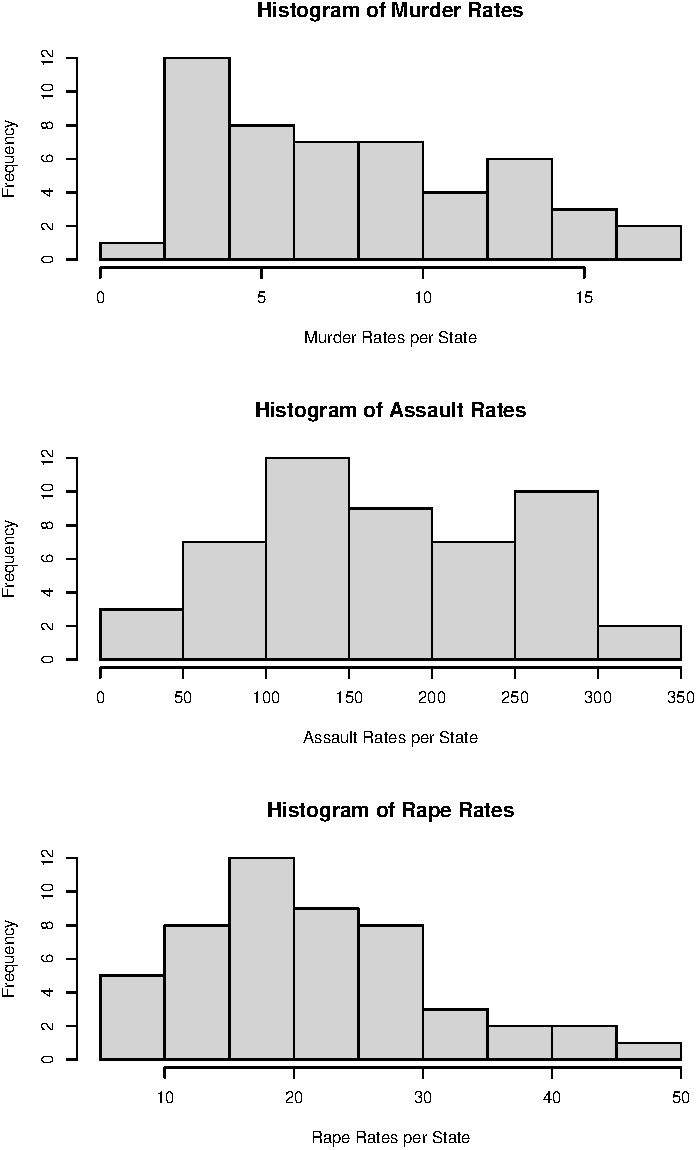
\includegraphics{Assignment-1-HarrisonMontoya_files/figure-latex/unnamed-chunk-8-1.pdf}

What does the command par do, in your own words (you can look this up by
asking R \texttt{?par})?

\emph{Answer:} The command par enables the statistician to set graphical
parameters for data in either a singular graph or multiple graphs.

What can you learn from plotting the histograms together?

\emph{Answer:} By plotting histograms together, you are able to compare
the data between different categories -- in this case, comparing the
differences in assault and murder rates per state, for example.
Additionally, you can gain a better understand of the data overall by
looking at it holistically instead of piece-by-piece.

\hypertarget{problem-8}{%
\subsubsection{Problem 8}\label{problem-8}}

In the console below (not in text), type
\texttt{install.packages("maps")} and press Enter, and then type
\texttt{install.packages("ggplot2")} and press Enter. This will install
the packages so you can load the libraries.

Run this code:

\begin{Shaded}
\begin{Highlighting}[]
\FunctionTok{library}\NormalTok{(}\StringTok{\textquotesingle{}maps\textquotesingle{}}\NormalTok{) }
\FunctionTok{library}\NormalTok{(}\StringTok{\textquotesingle{}ggplot2\textquotesingle{}}\NormalTok{) }

\FunctionTok{ggplot}\NormalTok{(dat, }\FunctionTok{aes}\NormalTok{(}\AttributeTok{map\_id=}\NormalTok{state, }\AttributeTok{fill=}\NormalTok{Murder)) }\SpecialCharTok{+} 
  \FunctionTok{geom\_map}\NormalTok{(}\AttributeTok{map=}\FunctionTok{map\_data}\NormalTok{(}\StringTok{"state"}\NormalTok{)) }\SpecialCharTok{+} 
  \FunctionTok{expand\_limits}\NormalTok{(}\AttributeTok{x=}\FunctionTok{map\_data}\NormalTok{(}\StringTok{"state"}\NormalTok{)}\SpecialCharTok{$}\NormalTok{long, }\AttributeTok{y=}\FunctionTok{map\_data}\NormalTok{(}\StringTok{"state"}\NormalTok{)}\SpecialCharTok{$}\NormalTok{lat)}
\end{Highlighting}
\end{Shaded}

What does this code do? Explain what each line is doing.

\emph{Answer:} This code is mapping the arrest rates of murder per
100,000 citizens per state. With this, we are able to see the salience
and prominence of arrest rates through a colored map of the United
States. The first line is using the data groups of ``state'' and
``Murder'' to construct aesthetic mapping in a ggplot, filling the map
with ``Murder'' rates. Next, the second line is the direction to map the
states, while the third line is expanding the x and y axes,
i.e.~longitude and latitude, in the graph.

\end{document}
